\section{LOS Coverage Map}\label{sec:los_map}
A point of interest regarding the project at hand is that Line-Of-Sight between the GS and the UA is fulfilled. As discussed in Chapter \ref{ch:frames} this model should take into account the followings:

\begin{itemize}
	\item Terrain elevation
	\item Curvature of the Earth
	\item Altitude of GS and UA
\end{itemize}

\subsection{Initial Step}
In this sense, a MATLAB script has been addressed which at first imports a Web Map Service (WMS) to load various maps and their topographic data. As an example a map which captures the area of Central Europe has been taken along with its terrain elevation levels as seen in Figure \ref{fig:before_map}.

\begin{figure}[H]
  \hfill
  \subfigure[Map Before Interaction]{
  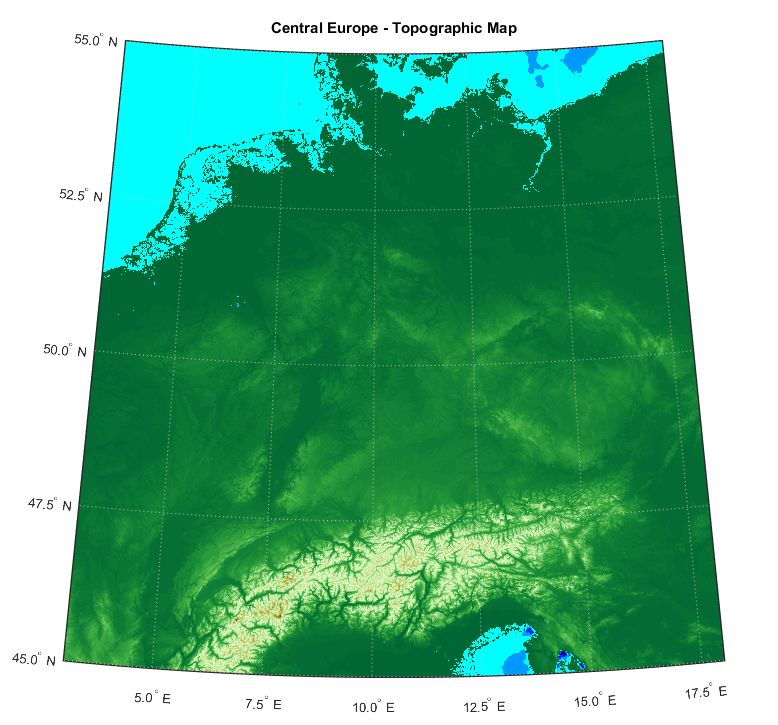
\includegraphics[scale=0.32]{figures/europe_map.png}
  \label{fig:before_map}}
  \hfill
  \subfigure[GS and UA Placement]{
  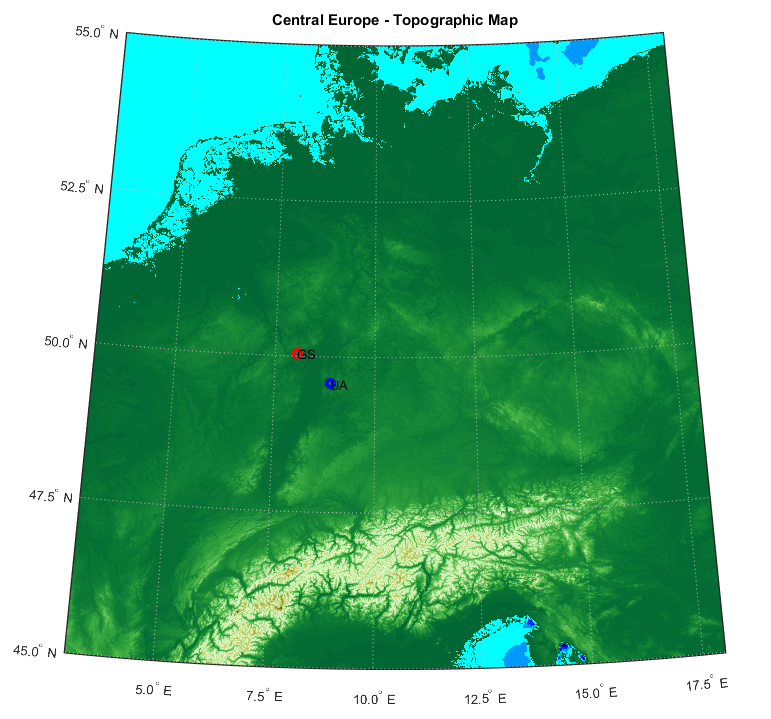
\includegraphics[scale=0.32]{figures/gs_ua_map.png}
  \label{fig:gs_uav_map}}
  \hfill
  \caption{Topographic Map of Central Europe}\label{fig:eu_map}
\end{figure}

\subsection{LOS Distance}
Given the map and its topographic data in Figure \ref{fig:before_map}, now it is possible to input the desired points for the GS (red) and the UA (blue) which gives as result in Figure \ref{fig:gs_uav_map}. As mentioned above, those parameters are taken into account in order to plot the LOS distance between the two points of interest. It can be observed in Figure \ref{fig:los_2p} that visibility is lost after 65 kilometers from the GS due to terrain elevation. On the other hand, in some parts of the distance it can be seen that the field of vision is regained, as a result of high terrain elevation around the 73th and 78th kilometer.

\begin{figure}[h]
	\centering
	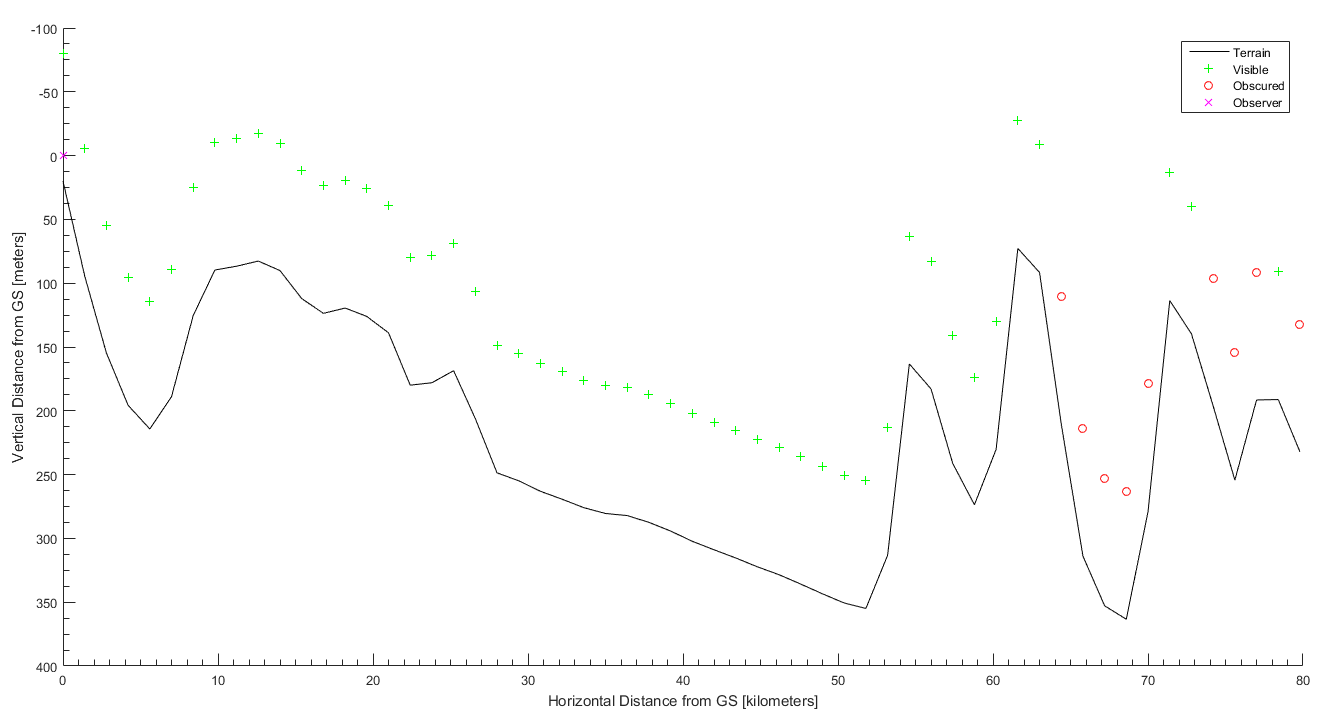
\includegraphics[scale=0.40]{figures/los_2p.png}
	\caption{LOS distance seen from local NED of GS \\ X axis - Distance [km] \\ Y axis - Altitude [m]}
   	\label{fig:los_2p}
\end{figure}

\subsection{Coverage Map}
Moving further, for the same map (Figure \ref{fig:before_map}), a location of the GS can be chosen, such that it will result into a visibility area (inside the white zone) as seen in Figure \ref{fig:los_area}. This area is also referred as the LOS coverage map and it takes into account the previously mentioned parameters.

\begin{figure}[h]
	\centering
	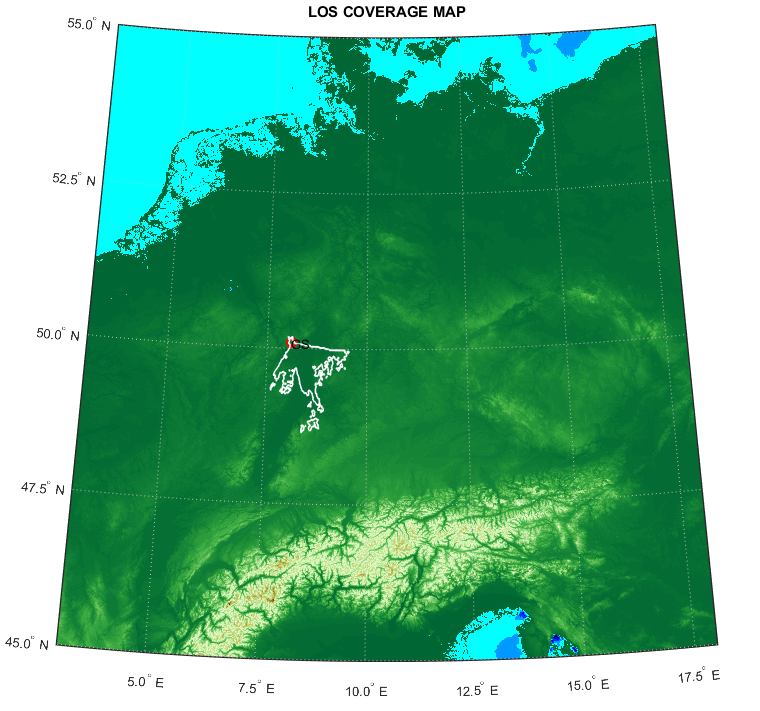
\includegraphics[scale=0.5]{figures/cov_map1.png}
	\caption{LOS Coverage Map from the GS}
   	\label{fig:los_area}
\end{figure}

It can be observed from Figure \ref{fig:los_area} that in some areas of the map there is no visibility, due to higher terrain elevation. This can be overcome by increasing the GS and/or UA altitude, such that we achieve visibility.  

\subsection{Working Principle}
Taking into account that a MATLAB script has been achieved, a thourough working principle has to be addressed in the following steps:
\begin{itemize}
	\item Import topography map 
	\item Input GS and UA altitudes
	\item Choose (click) GS and UA locations on map in order to plot LOS distance
	\item Choose (click) location of the GS in order to plot the LOS coverage map
\end{itemize}